% This file is only used to generate the figure to be included
% This does not need to be compiled each time
% Do not attempt to include this in the main document, it will break LaTeX!

\documentclass{standalone}

\usepackage{tikz}
\usetikzlibrary{automata,positioning}

\begin{document}
    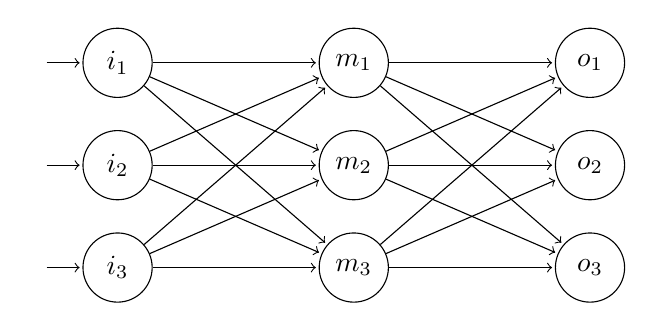
\begin{tikzpicture}[shorten >=1pt,node distance=1.3cm and 3cm,on grid,auto,initial text={}] 
    \node[state,initial] (i1) {$i_1$};
    \node[state,initial] (i2) [below=of i1] {$i_2$}; 
    \node[state,initial] (i3) [below=of i2] {$i_3$}; 

    \node[state] (h11) [right=of i1] {$m_1$};
    \node[state] (h12) [below=of h11] {$m_2$}; 
    \node[state] (h13) [below=of h12] {$m_3$}; 

    \node[state] (hb1) [right=of h11] {$o_1$};
    \node[state] (hb2) [below=of hb1] {$o_2$}; 
    \node[state] (hb3) [below=of hb2] {$o_3$}; 

    \path[->] 
    (i1) edge node {} (h11) (i2) edge node {} (h11)
    (i1) edge node {} (h12) (i2) edge node {} (h12)
    (i1) edge node {} (h13) (i2) edge node {} (h13)
    (i3) edge node {} (h11) (h11) edge node {} (hb1)
    (i3) edge node {} (h12) (h11) edge node {} (hb2)
    (i3) edge node {} (h13) (h11) edge node {} (hb3)
    (h12) edge node {} (hb1) (h13) edge node {} (hb1)
    (h12) edge node {} (hb2) (h13) edge node {} (hb2)
    (h12) edge node {} (hb3) (h13) edge node {} (hb3)

    ;
    \end{tikzpicture}
\end{document}